\begin{titlepage}

 \begin{figure}
  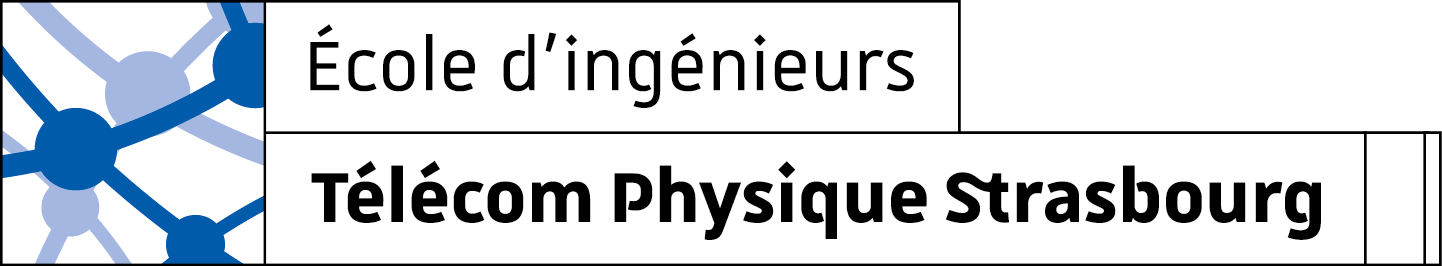
\includegraphics[width=7cm]{logos/tps_logo.png}
  \hfill
  
\includegraphics[width=4cm]{logos/unistra_logo.png}
 \end{figure}

 \hfill
 \begin{minipage}{3cm}
  \begin{flushright}
   \vspace{3cm}
   PLASSE, Jonathan\\
   Promo 2020\\
   Année 2018 -- 2019
  \end{flushright}
 \end{minipage}

 \vspace{3.5cm}

 \begin{center}
  \hrulefill \\
  \vspace{0.3cm}
  \Large{Diplôme d’ingénieur -- Télécom Physique Strasbourg\\
   Mémoire de stage de 2\textsuperscript{ème} année
  }\\
  \vspace{0,2cm}
  \textsc{\textbf{\guillemotleft \ \normalsize{\textbf{\large{Hardware and Software Development for Aerial Robot Swarms}}} \ \Large{\guillemotright}}} \\
  \hrulefill

  \vspace{0.7cm}
 \end{center}

 \vfill
 \begin{figure}[h!]
  \hspace{0.29cm}
  
\includegraphics[width=2cm]{logos/vub_logo.jpg}
 \end{figure}
 \begin{minipage}{8cm}
  \textbf{Vrije Universiteit Brussel}\\
  Pleinlaan 2 | Building Z | 2nd floor\\
  B-1050 Brussels | Belgium
 \end{minipage} \hfill
 \begin{minipage}{7cm}
  \begin{flushright}
   Bryan Convens\\
   \texttt{Bryan.Convens@vub.be}\\
   +32 7 00 00 00 00\\ \vspace{0.2cm}
   Du 10 June au 30 August 2019
  \end{flushright}
 \end{minipage}

\end{titlepage}


\chapter*{Acknowledgment}\pagenumbering{roman}
I would like to thanks everyone at Brubotics for their welcoming attitude,
the activities passed together and the wonderful conversations.
In particular, I would like to thank Professor Bram Vanderborght for accepting me at Brubotics,
Bryan Convens for mentoring me, Pablo for his kindness and showing me around,
Kelly, Helen, Joris, Stein, Jarl, Vincent, Kevin, I will never forget the canoe, the football match and the Rollerblade parade.

\chapter*{Abstracts}
{\color{red}Improve the phrasing}
\section*{Résumé Français}
Le but de ce stage a été de mettre en place une infrastructure de développement pour pouvoir tester sur un groupe de drones algorithmes de contrôle en utilisant des communications sans fil à hautes bandes passantes, de la capture de mouvement et ROS.

Plusieurs solutions de logiciels d'autopilote ont été explorées en parallèle du contrôleur de vol. Le choix s'est porté sur ArduPilot comme autopilote et Raspberry Pi Navio2 comme contrôleur de vol et ordinateur de bord.

Il a fallu ensuite choisir les différents composants du drone en s'assurant que l'ensemble remplisse le cahier des charges, que les différents composants soient compatibles entre eux.

Un guide détaillé a été rédigé pour construire le drone et le paramétrer pour le faire voler.

Des extensions ont ensuite été apportées à la configuration de base pour pouvoir communiquer à plusieurs drones en même temps.


\section*{English Asbtract}
The idea of this internship has been to create a framework to test control algorithms on a swarm of drones using high bandwidth wireless communication, motion capture, and ROS.

Exploring the possible solutions of autopilot software to see which one would be the best fit for this project. ArduPilot was chosen as autopilot software and Raspberry Pi Navio2 as flight controller and companion computer.

Designing a drone that can fly with a companion computer and assuring it is compatible with the chosen autopilot software.

Building a drone and creating instructions on how to build the drones.

Configuring and testing a drone without making a change to the autopilot software.

Making extensions to the project to communicate with multiple drones.
